%==============================================================================
% Chapitre 49 - Classification des munitions
%==============================================================================

\section{Introduction}

Les munitions existent sous une très grande variété de formes.

Cette diversité résulte des nombreux usages auxquels elles sont destinées :

\begin{itemize}
    \item défense ;
    \item usage militaire ;
    \item chasse ;
    \item tir sportif ;
    \item entraînement ;
    \item applications techniques.
\end{itemize}

Une classification permet de mieux comprendre leurs caractéristiques et leurs
domaines d'emploi.

\begin{aretenir}

Une munition est généralement conçue pour répondre à un besoin précis.

\end{aretenir}

\section{Critères de classification}

Les munitions peuvent être classées selon plusieurs critères :

\begin{itemize}
    \item leur usage ;
    \item leur calibre ;
    \item leur mode de fonctionnement ;
    \item leur projectile ;
    \item leur énergie ;
    \item leur destination.
\end{itemize}

Une même munition peut appartenir simultanément à plusieurs catégories.

\begin{figure}[htbp]
\centering

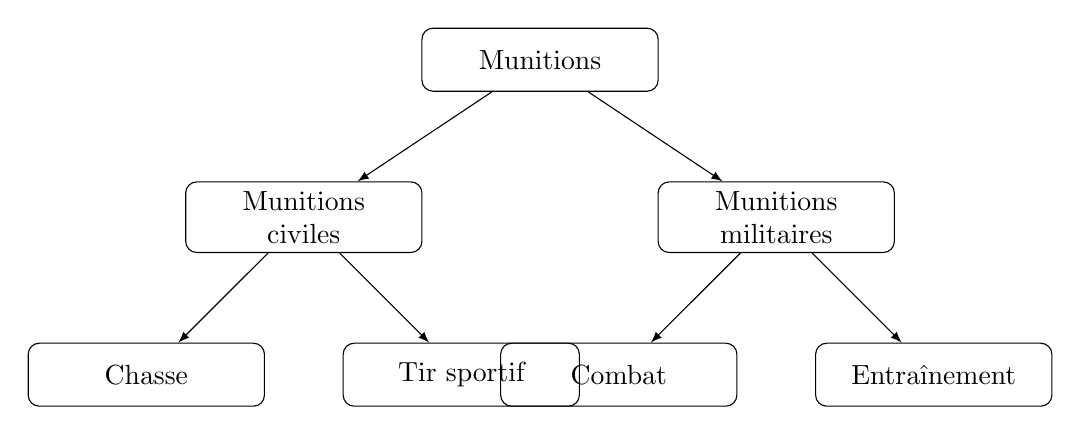
\begin{tikzpicture}[
every node/.style={
draw,
rounded corners,
align=center,
minimum width=3cm,
minimum height=8mm
}
]

\node (M) at (0,0) {Munitions};

\node (C) at (-3,-2) {Munitions\\civiles};
\node (Mil) at (3,-2) {Munitions\\militaires};

\node (Ch) at (-5,-4) {Chasse};
\node (Sp) at (-1,-4) {Tir sportif};

\node (Co) at (1,-4) {Combat};
\node (En) at (5,-4) {Entraînement};

\draw[-latex] (M) -- (C);
\draw[-latex] (M) -- (Mil);

\draw[-latex] (C) -- (Ch);
\draw[-latex] (C) -- (Sp);

\draw[-latex] (Mil) -- (Co);
\draw[-latex] (Mil) -- (En);

\end{tikzpicture}

\caption{Exemple simplifié de classification des munitions.}
\label{fig:classification_munitions}

\end{figure}


\section{Munitions militaires}

Les munitions militaires sont destinées aux forces armées.

Leur conception privilégie généralement :

\begin{itemize}
    \item la fiabilité ;
    \item la robustesse ;
    \item la standardisation ;
    \item la compatibilité logistique.
\end{itemize}

Elles répondent souvent à des spécifications strictes.

\section{Munitions civiles}

Les munitions civiles regroupent de nombreuses catégories :

\begin{itemize}
    \item chasse ;
    \item tir sportif ;
    \item tir récréatif ;
    \item défense.
\end{itemize}

Leurs caractéristiques varient fortement selon l'application.

\section{Munitions de chasse}

Les munitions de chasse sont conçues pour produire des effets adaptés au
gibier recherché.

Le projectile peut être optimisé pour :

\begin{itemize}
    \item l'expansion ;
    \item la pénétration ;
    \item le transfert d'énergie ;
    \item la limitation des ricochets.
\end{itemize}

\section{Munitions de tir sportif}

Le tir sportif privilégie généralement :

\begin{itemize}
    \item la précision ;
    \item la régularité ;
    \item la reproductibilité.
\end{itemize}

Les munitions utilisées sont souvent fabriquées avec des tolérances très
strictes.

\section{Munitions d'entraînement}

Les munitions d'entraînement visent principalement :

\begin{itemize}
    \item la réduction des coûts ;
    \item la sécurité ;
    \item la répétition des exercices.
\end{itemize}

Elles reproduisent souvent le comportement des munitions opérationnelles.

\section{Munitions de défense}

Les munitions de défense sont destinées à l'autoprotection ou aux forces de
l'ordre.

Leurs caractéristiques dépendent du cadre légal et des contraintes
opérationnelles.

\section{Classification selon le projectile}

Une autre méthode consiste à classer les munitions selon leur projectile.

On distingue notamment :

\begin{itemize}
    \item les projectiles blindés ;
    \item les projectiles expansifs ;
    \item les projectiles perforants ;
    \item les projectiles traceurs ;
    \item les projectiles incendiaires.
\end{itemize}

\section{Classification selon l'énergie}

Les munitions peuvent également être regroupées selon leur énergie.

On parle parfois :

\begin{itemize}
    \item de faible puissance ;
    \item de puissance intermédiaire ;
    \item de forte puissance.
\end{itemize}

Ces catégories ne possèdent pas de définition universelle.

\section{Classification selon la vitesse}

Selon leur vitesse initiale, certaines munitions sont qualifiées de :

\begin{itemize}
    \item subsoniques ;
    \item transsoniques ;
    \item supersoniques.
\end{itemize}

Cette distinction influence fortement la balistique extérieure.

\begin{figure}[htbp]
\centering

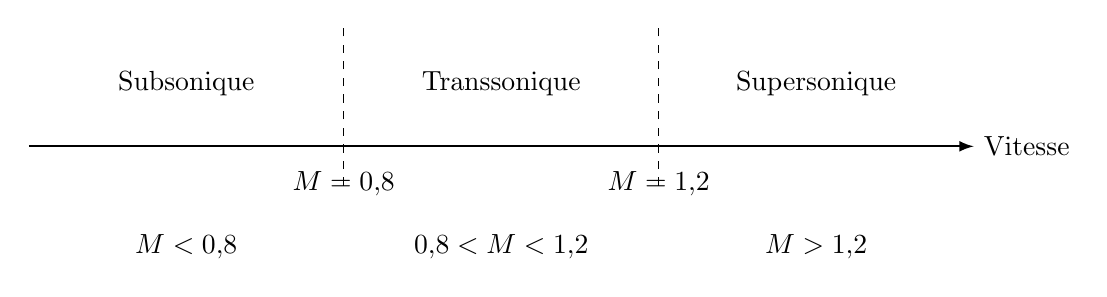
\begin{tikzpicture}[scale=1]

% Axe
\draw[-latex,thick]
(0,0)
--
(12,0)
node[right] {Vitesse};

% Séparations
\draw[dashed]
(4,-0.5)
--
(4,1.5);

\draw[dashed]
(8,-0.5)
--
(8,1.5);

% Zones
\node at (2,0.8)
{Subsonique};

\node at (6,0.8)
{Transsonique};

\node at (10,0.8)
{Supersonique};

% Bornes
\node[below]
at (4,-0.2)
{$M=0{,}8$};

\node[below]
at (8,-0.2)
{$M=1{,}2$};

% Explications
\node[below]
at (2,-1)
{$M<0{,}8$};

\node[below]
at (6,-1)
{$0{,}8<M<1{,}2$};

\node[below]
at (10,-1)
{$M>1{,}2$};

\end{tikzpicture}

\caption{Classification simplifiée selon le nombre de Mach.}
\label{fig:classification_vitesse}

\end{figure}

\section{Classification selon le type d'arme}

Certaines munitions sont conçues pour :

\begin{itemize}
    \item les armes de poing ;
    \item les fusils ;
    \item les carabines ;
    \item les armes automatiques ;
    \item les armes d'artillerie.
\end{itemize}

\section{Munitions à balle et à grenaille}

Dans les armes lisses, on distingue généralement :

\begin{itemize}
    \item les cartouches à balle unique ;
    \item les cartouches à grenaille.
\end{itemize}

Leur comportement balistique est très différent.

\section{Munitions spéciales}

Certaines munitions répondent à des besoins particuliers :

\begin{itemize}
    \item traçantes ;
    \item perforantes ;
    \item incendiaires ;
    \item d'exercice ;
    \item à blanc.
\end{itemize}

Leurs caractéristiques seront détaillées dans des chapitres ultérieurs.

\section{Pourquoi autant de variantes ?}

Chaque usage impose des contraintes différentes.

Une munition idéale pour le tir de précision n'est pas nécessairement adaptée :

\begin{itemize}
    \item à la chasse ;
    \item à l'entraînement ;
    \item à un usage militaire.
\end{itemize}

Cette diversité explique le grand nombre de cartouches existantes.

\section{Vers les munitions militaires}

Parmi toutes les catégories étudiées, les munitions militaires occupent une
place particulière en raison de leur influence historique sur le développement
de nombreuses cartouches modernes.

Le chapitre suivant leur sera consacré.

\section{À retenir}

\begin{aretenir}

\begin{itemize}
    \item Les munitions peuvent être classées selon de nombreux critères.
    \item Une même cartouche peut appartenir à plusieurs catégories.
    \item L'usage recherché influence fortement la conception.
    \item Les projectiles constituent un critère de classification majeur.
    \item La diversité des munitions reflète la diversité des besoins.
\end{itemize}

\end{aretenir}
